\documentclass{article}
\usepackage{graphicx}
\usepackage{hyperref}
\usepackage{amsmath}
\usepackage{booktabs}
\usepackage{geometry}
\geometry{a4paper, margin=1in}

\title{Dynamic Array Scaling: Formula A Progress Report}
\date{\today}

\begin{document}
\maketitle

\section{Introduction}
Dynamic arrays traditionally use a fixed growth factor (e.g., $2.0\times$ in C++ or $1.5\times$ in Java) upon reallocation. While simple, these fixed strategies often result in significant memory waste at large capacities. The purpose of this research is to evaluate adaptive growth factors that gracefully decay as capacity increases, thus conserving memory, while avoiding an excessive number of array resizes and element copies.

This report summarizes the testing and evaluation of \textbf{Formula A: Logarithmic Adaptive Growth}. The evaluation was split into Phase 1 (Constant $\alpha$) and Phase 2 (Workload-Aware Logarithmic $\alpha$), as documented in our theoretical models (\texttt{new\_formulas.md}).

\section{Phase 1: Constant Alpha Baseline}
In Phase 1, the scaling factor $\alpha$ is kept constant. The growth factor solely depends on the current capacity $C$:
\begin{equation}
g(C) = \min\left(g_{\max}, \max\left(g_{\min}, 1 + \frac{\alpha}{\ln(C+\beta)}\right)\right)
\end{equation}

\subsection{Results Summary (N = 1,000,000)}
For 1,000,000 insertions, the adaptive formula significantly outperformed fixed growth in terms of memory waste. \texttt{FormulaA(a=3.5, b=10)} provided the best balance of speed and copy cost among the adaptive methods, while \texttt{FormulaA(a=1.5, b=2)} achieved the lowest absolute waste.

\begin{table}[h!]
    \centering
    \begin{tabular}{lrrr}
        \toprule
        \textbf{Strategy} & \textbf{Resizes} & \textbf{Total Copied} & \textbf{Waste (\%)} \\
        \midrule
        Fixed $2.0\times$ & 17 & 1,310,710 & 23.71\% \\
        Fixed $1.5\times$ & 29 & 2,430,972 & 17.73\% \\
        FormulaA ($a=3.5, b=10$) & 32 & 3,951,990 & 7.69\% \\
        FormulaA ($a=1.5, b=2$) & 67 & 8,509,374 & 0.04\% \\
        \bottomrule
    \end{tabular}
    \caption{Key Performance Metrics for Phase 1 at 1,000,000 Insertions.}
    \label{tab:phase1}
\end{table}

\begin{figure}[h!]
    \centering
    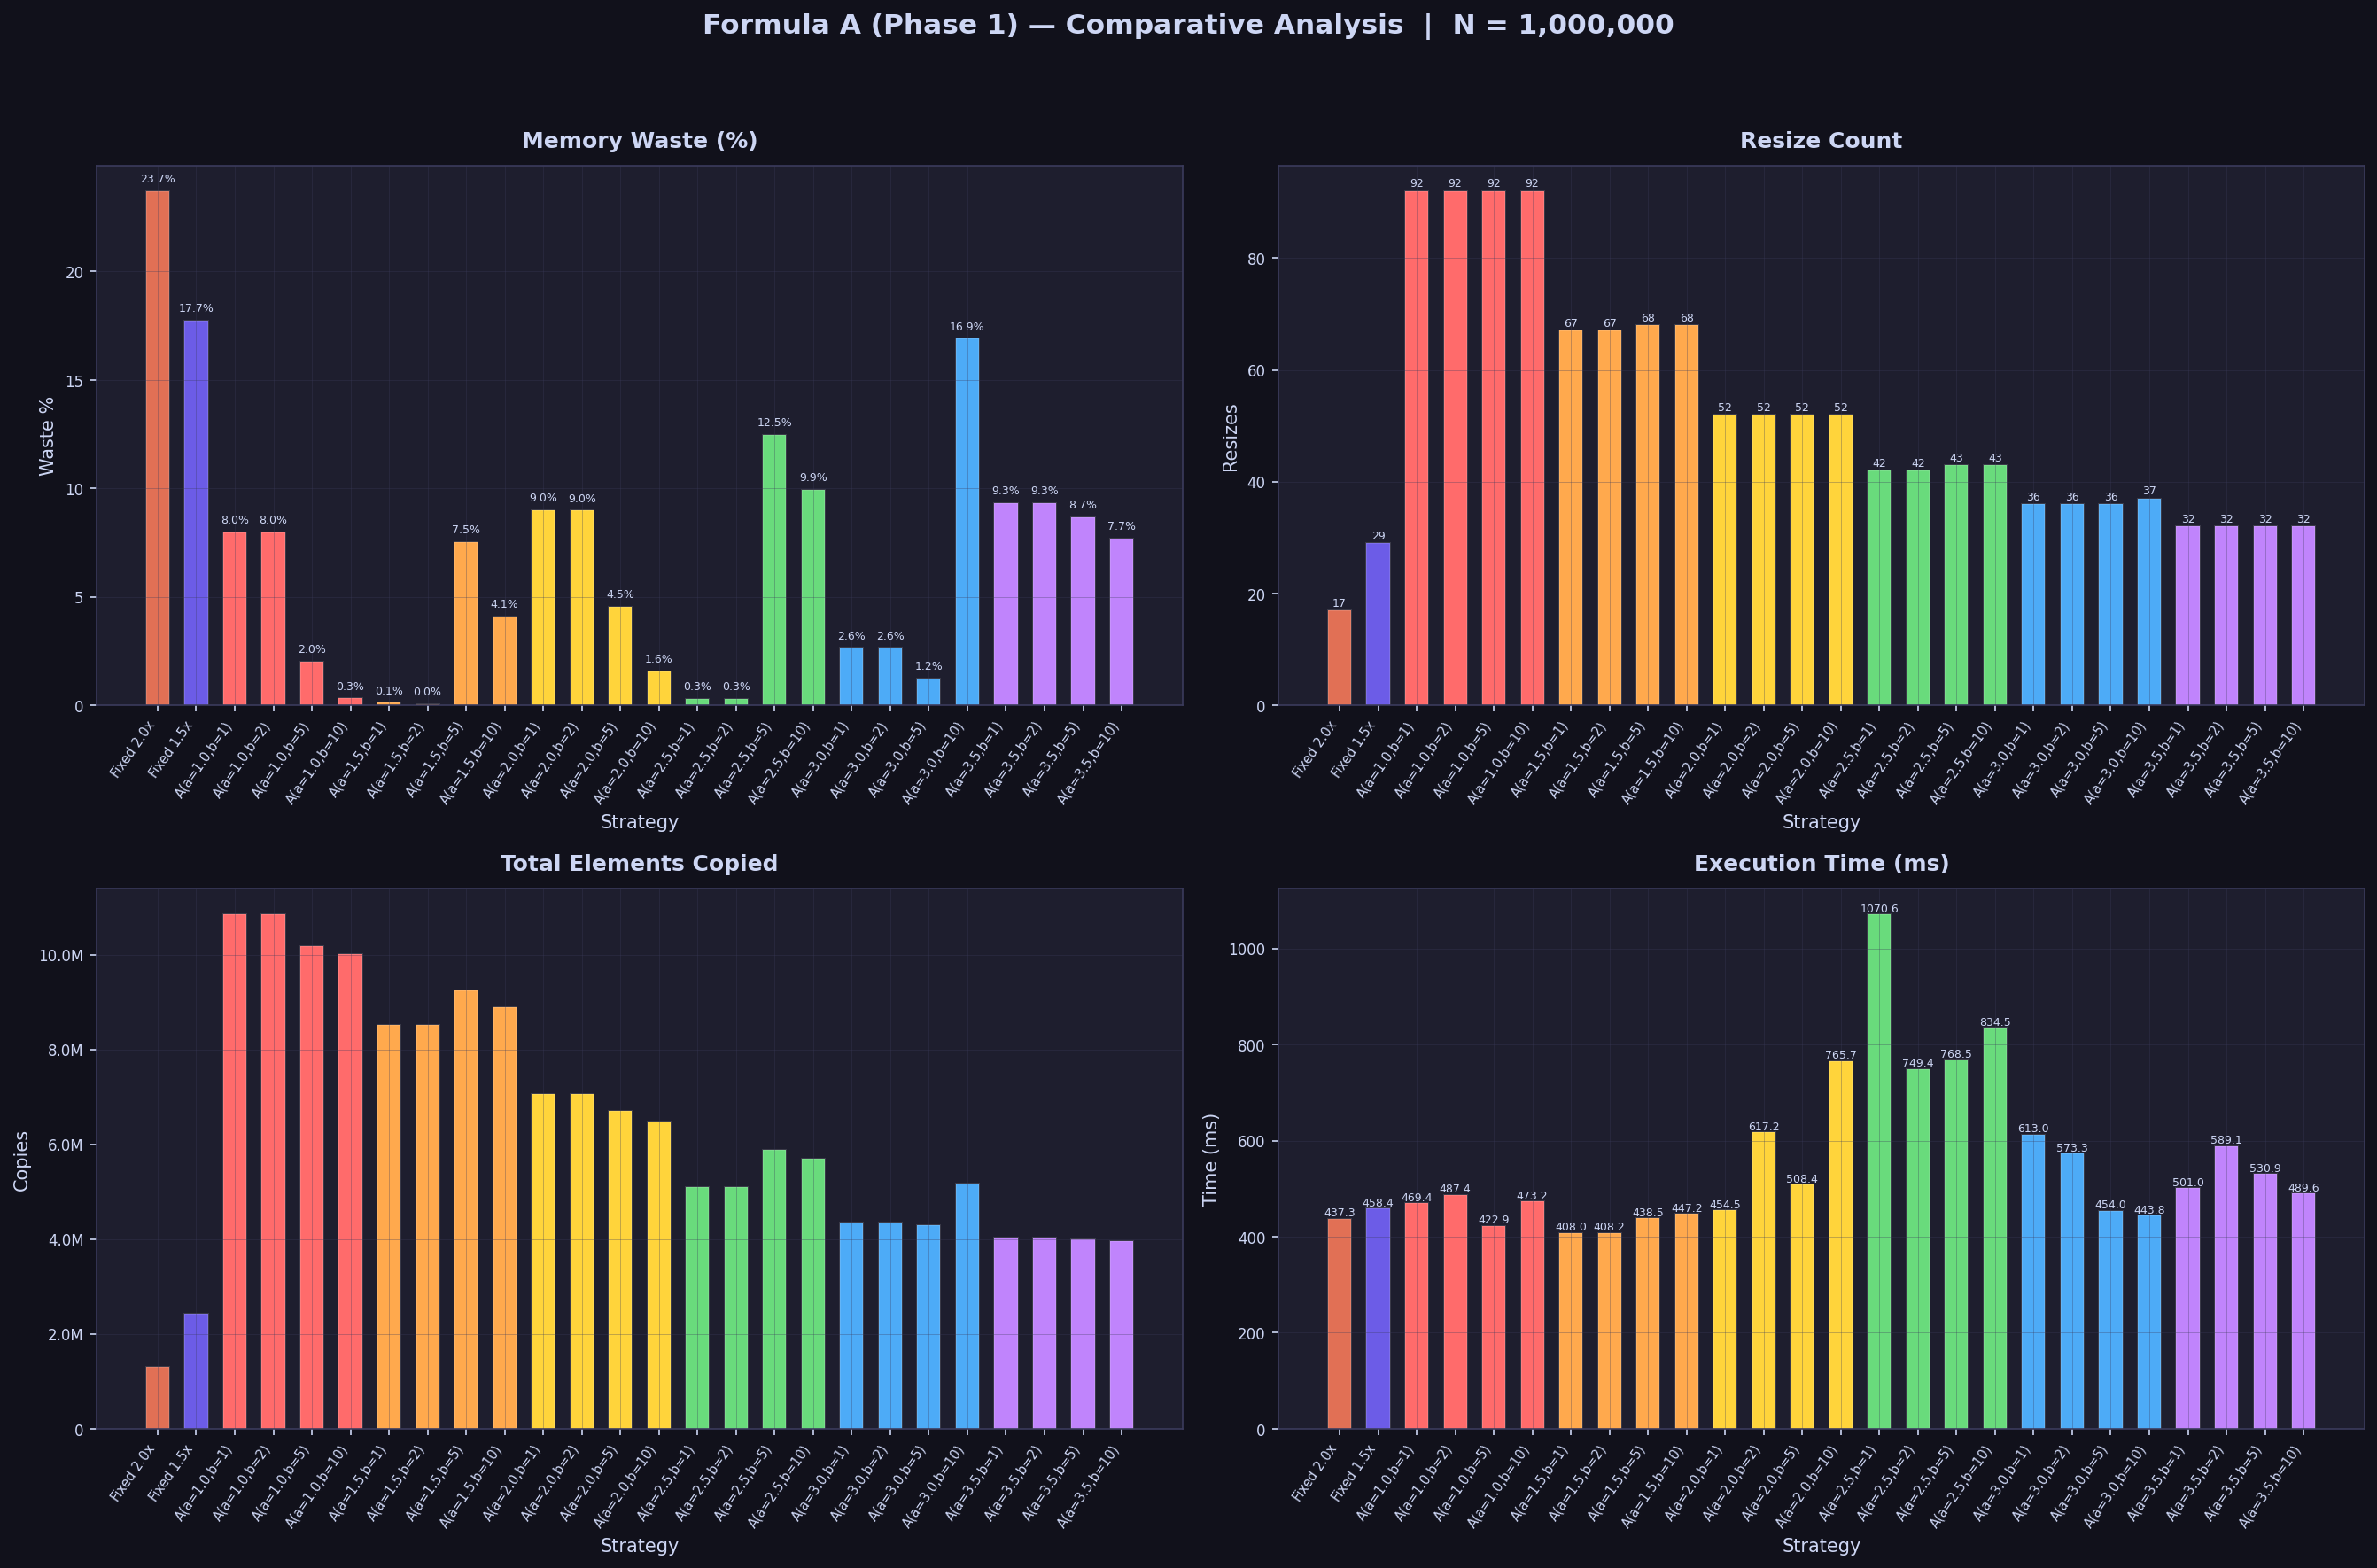
\includegraphics[width=0.9\textwidth]{../form_A_phas_A/formula_a_comparison_1000000_v2.png}
    \caption{Phase 1: Memory Waste and Copy Cost comparison at $N = 1,000,000$.}
    \label{fig:phase1_1m}
\end{figure}

\clearpage

\section{Phase 2: Workload-Aware Logarithmic Alpha}
In Phase 2, we introduce workload-awareness by adjusting the scaling factor based on the insertion velocity $v = \frac{\Delta N}{\Delta t}$.

Based on early testing, a linear scalar ($\alpha(v) = \alpha_{base} + kv$) clipped to the maximum growth factor ($g_{\max} = 2.0$) too abruptly during high-velocity workloads. Thus, we adopted a \textbf{logarithmic scaling mechanism} for velocity:
\begin{equation}
\alpha(v) = 3.0 + k \ln(1 + v)
\end{equation}
Yielding the final growth equation:
\begin{equation}
g(C, v) = \min\left(g_{\max}, \max\left(g_{\min}, 1 + \frac{3.0 + k \ln(1+v)}{\ln(C+5)}\right)\right)
\end{equation}

\subsection{Results Summary (N = 1,000,000)}
We subjected the Phase 2 formula to four distinct insertion patterns. The table below highlights the performance of the best configurations under Constant ($v=10$), Accelerating ($1 \to 1000$), and Spiky velocities.

\begin{table}[h!]
    \centering
    \begin{tabular}{llrrr}
        \toprule
        \textbf{Pattern} & \textbf{Strategy} & \textbf{Resizes} & \textbf{Total Copied} & \textbf{Waste (\%)} \\
        \midrule
        \textbf{Constant ($v=10$)} & Fixed $2.0\times$ & 17 & 1,310,710 & 23.71\% \\
        & Phase 1 Base ($a=3, b=5$) & 36 & 4,291,665 & 1.22\% \\
        & Phase 2 ($k=1.0$) & 23 & 2,366,269 & 1.06\% \\
        \midrule
        \textbf{Accelerating ($1 \to 1000$)} & Fixed $2.0\times$ & 17 & 1,310,710 & 23.71\% \\
        & Phase 1 Base ($a=3, b=5$) & 36 & 4,291,665 & 1.22\% \\
        & Phase 2 ($k=2.0$) & 26 & 2,636,049 & 3.79\% \\
        \midrule
        \textbf{Spiky} & Phase 1 Base ($a=3, b=5$) & 36 & 4,291,665 & 1.22\% \\
        & Phase 2 ($k=1.0$) & 21 & 2,572,485 & 12.16\% \\
        \bottomrule
    \end{tabular}
    \caption{Key Performance Metrics for Phase 2 at 1,000,000 Insertions under varying patterns.}
    \label{tab:phase2}
\end{table}

\begin{figure}[h!]
    \centering
    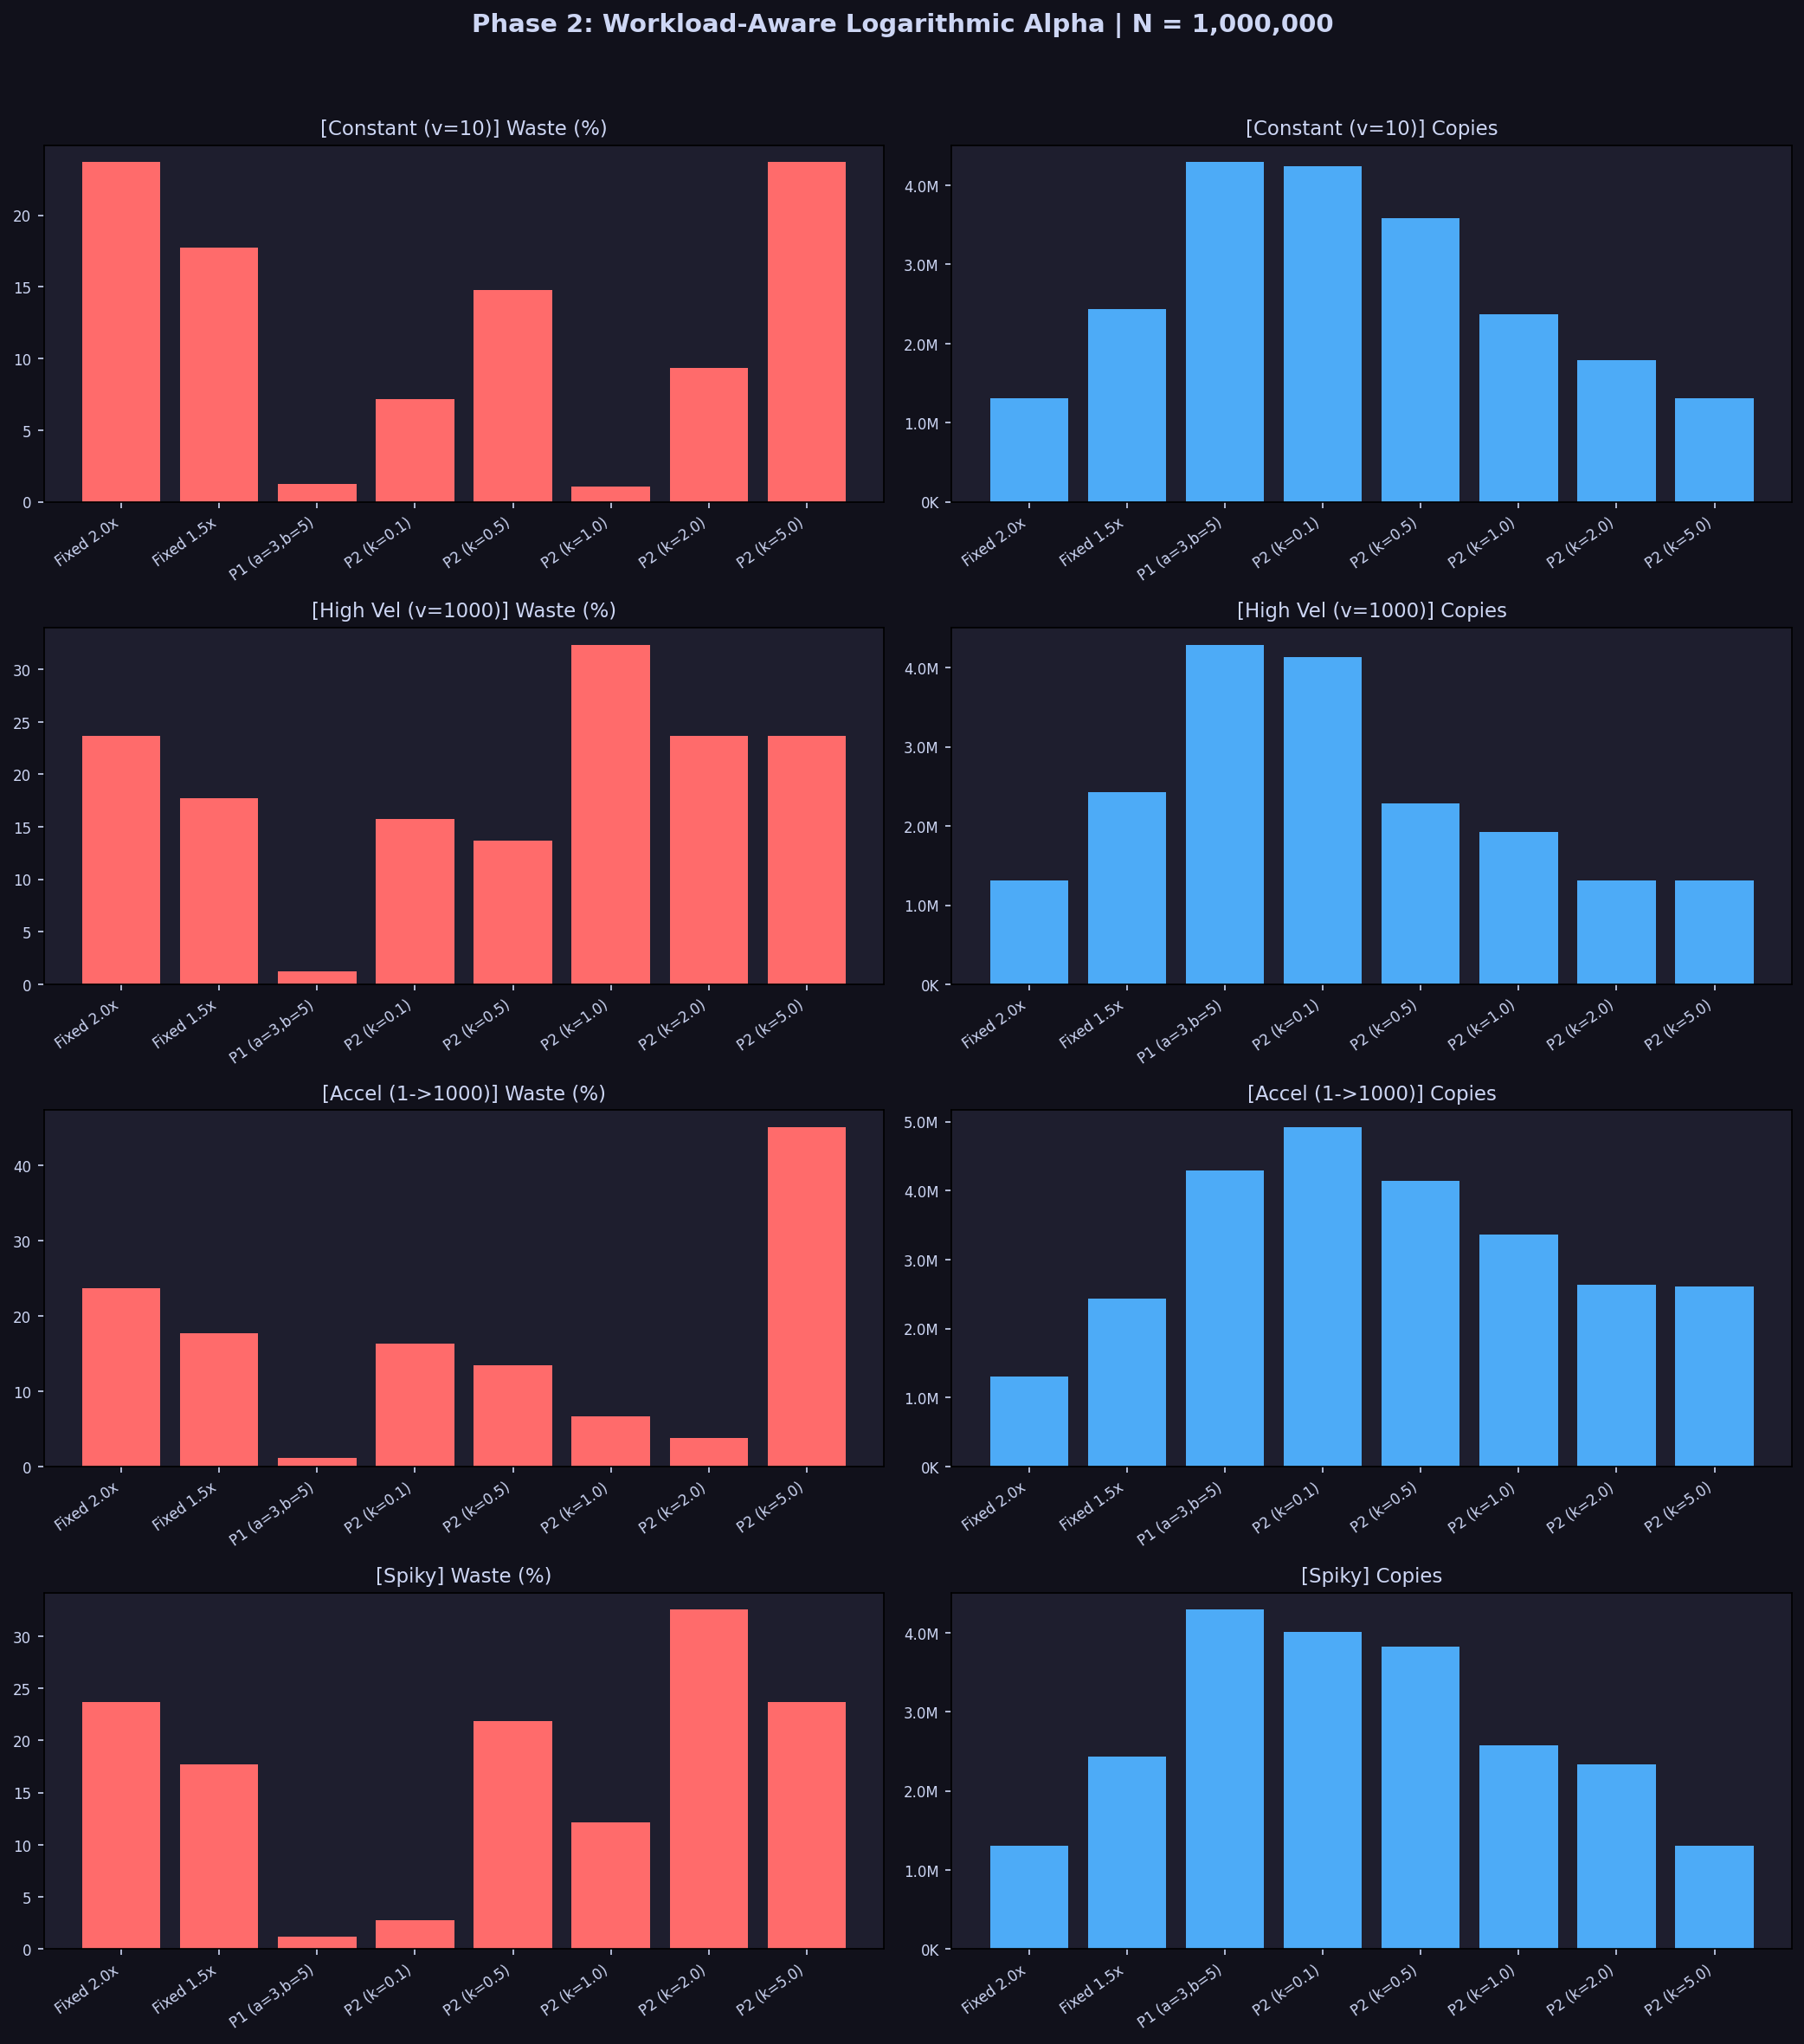
\includegraphics[width=0.9\textwidth]{../form_A_phase_2/phase2_comparison_1000000.png}
    \caption{Phase 2: Workload-Aware Scaling mapped across different insertion patterns at $N = 1,000,000$.}
    \label{fig:phase2_1m}
\end{figure}

\clearpage

\section{Formula B Phase 1: Standard Harmonic Growth}
In Formula B, the growth factor is determined by the resize history (the number of resize operations $k$). We generalize the harmonic sequence by introducing a tunable numerator parameter $c$:
\begin{equation}
g(k) = \min\left(g_{\max}, \max\left(g_{\min}, 1 + \frac{c}{k}\right)\right)
\end{equation}

\subsection{Results Summary (N = 1,000,000)}
The harmonic sequence strategy yields extremely tight memory bounds, but the aggressive decay of the growth factor causes an unacceptably high number of element copies compared to Formula A and fixed baselines.

\begin{table}[h!]
    \centering
    \begin{tabular}{lrrr}
        \toprule
        \textbf{Strategy} & \textbf{Resizes} & \textbf{Total Copied} & \textbf{Waste (\%)} \\
        \midrule
        Fixed $2.0\times$ & 17 & 1,310,710 & 23.71\% \\
        Formula A ($a=3.5, b=10$) & 32 & 3,951,990 & 7.69\% \\
        Formula B ($c=1.0$) & 106 & 10,020,732 & 0.21\% \\
        Formula B ($c=3.0$) & 71 & 10,803,264 & 7.90\% \\
        Formula B ($c=5.0$) & 37 & 6,644,767 & 7.19\% \\
        \bottomrule
    \end{tabular}
    \caption{Key Performance Metrics for Formula B Phase 1 at 1,000,000 Insertions.}
    \label{tab:form_b_phase1}
\end{table}

\begin{figure}[h!]
    \centering
    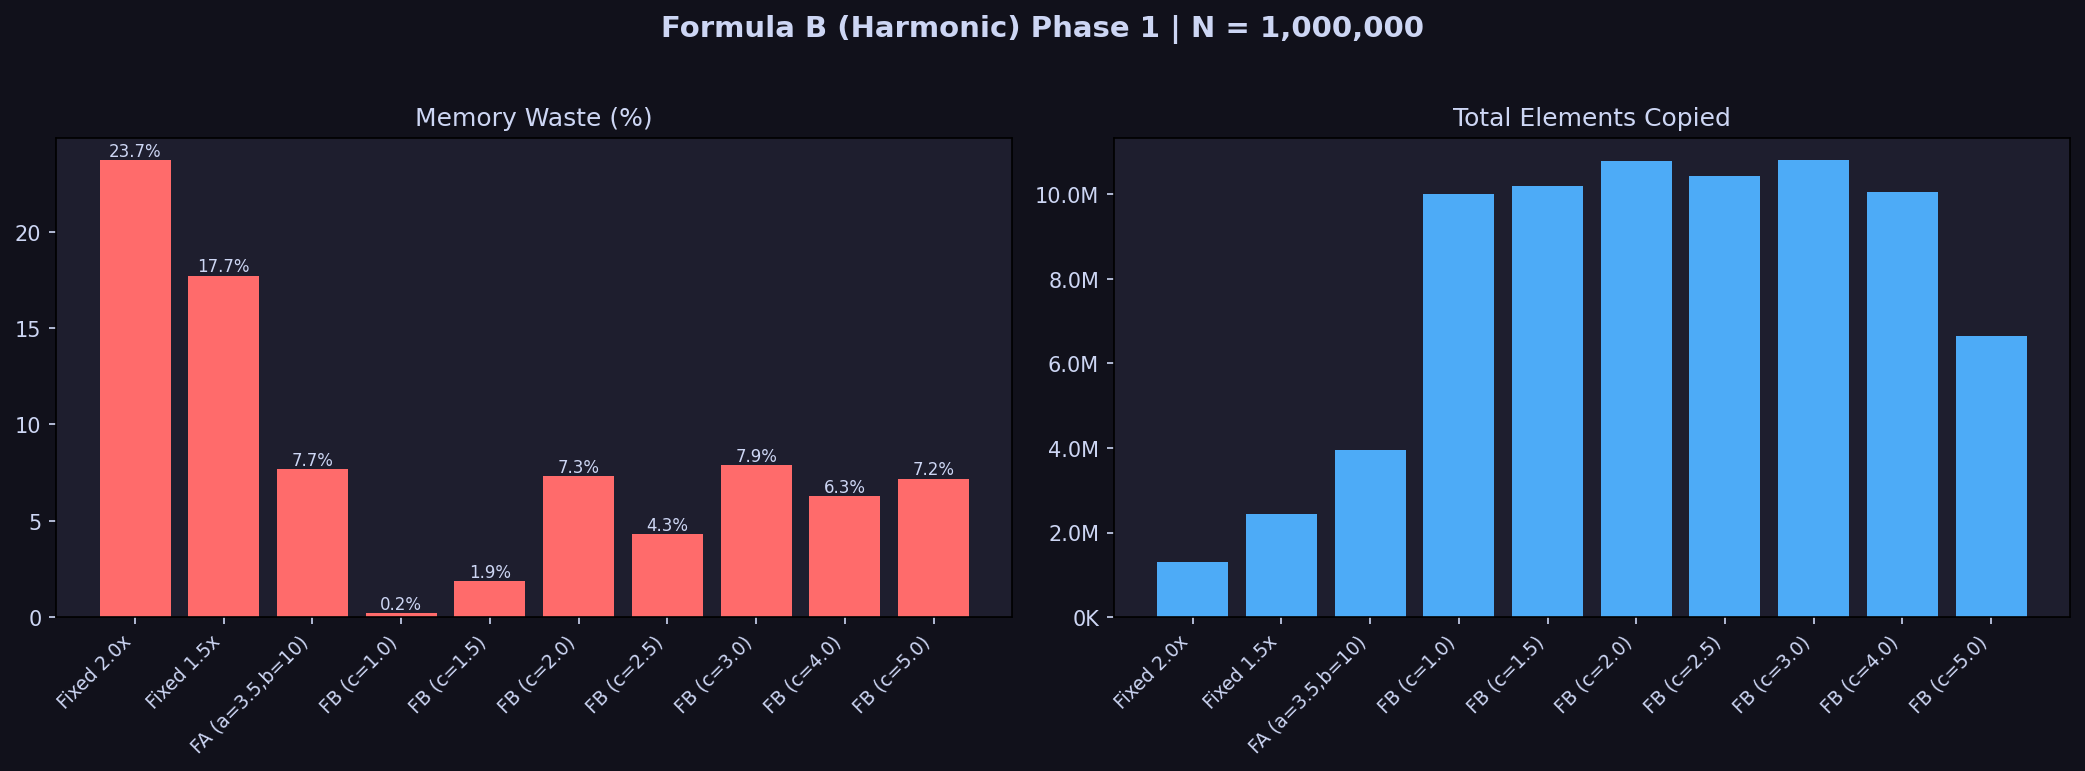
\includegraphics[width=0.9\textwidth]{../form_B_phas_1/formula_b_comparison_1000000.png}
    \caption{Formula B Phase 1: Memory Waste and Copy Cost comparison at $N = 1,000,000$.}
    \label{fig:form_b_phase1_1m}
\end{figure}

The pure harmonic growth decays too rapidly for standard workloads. While memory waste is exceptionally low (reaching $0.21\%$ for $c=1.0$), it results in severe resize thrashing ($>10$ million copies). This validates the necessity of integrating workload-awareness into the numerator (Phase 2) to flatten the decay curve during sustained insertions.

\clearpage

\section{Formula B Phase 2: Workload-Aware Harmonic Growth}
To address the extreme resize thrashing identified in Phase 1, insertion velocity $v$ was introduced into the numerator of the harmonic sequence. This allows the growth factor to increase dynamically during bursts, counteracting the rapid harmonic decay. The formula is parameterized by workload sensitivity $\lambda$:
\begin{equation}
g(k,v) = \min\left(g_{\max}, \max\left(g_{\min}, 1 + \frac{1 + \lambda \ln(1+v)}{k}\right)\right)
\end{equation}

\subsection{Results Summary (N = 1,000,000)}
The addition of logarithmic velocity scaling successfully transforms Formula B into an incredibly elastic strategy that perfectly manages Spiky and High-Velocity workloads.

\begin{table}[h!]
    \centering
    \begin{tabular}{llrrr}
        \toprule
        \textbf{Pattern} & \textbf{Strategy} & \textbf{Resizes} & \textbf{Total Copied} & \textbf{Waste (\%)} \\
        \midrule
        \textbf{High Vel ($v=1000$)} & Fixed $2.0\times$ & 17 & 1,310,710 & 23.71\% \\
        & Phase 1 Base ($c=5.0$) & 37 & 6,644,767 & 7.19\% \\
        & Phase 2 ($\lambda=2.0$) & 17 & 1,280,657 & 14.83\% \\
        \midrule
        \textbf{Spiky} & Fixed $2.0\times$ & 17 & 1,310,710 & 23.71\% \\
        & Phase 1 Base ($c=5.0$) & 37 & 6,644,767 & 7.19\% \\
        & Phase 2 ($\lambda=5.0$) & 17 & 1,209,830 & 5.09\% \\
        \bottomrule
    \end{tabular}
    \caption{Key Performance Metrics for Formula B Phase 2 at 1,000,000 Insertions under varying patterns.}
    \label{tab:form_b_phase2}
\end{table}

\begin{figure}[h!]
    \centering
    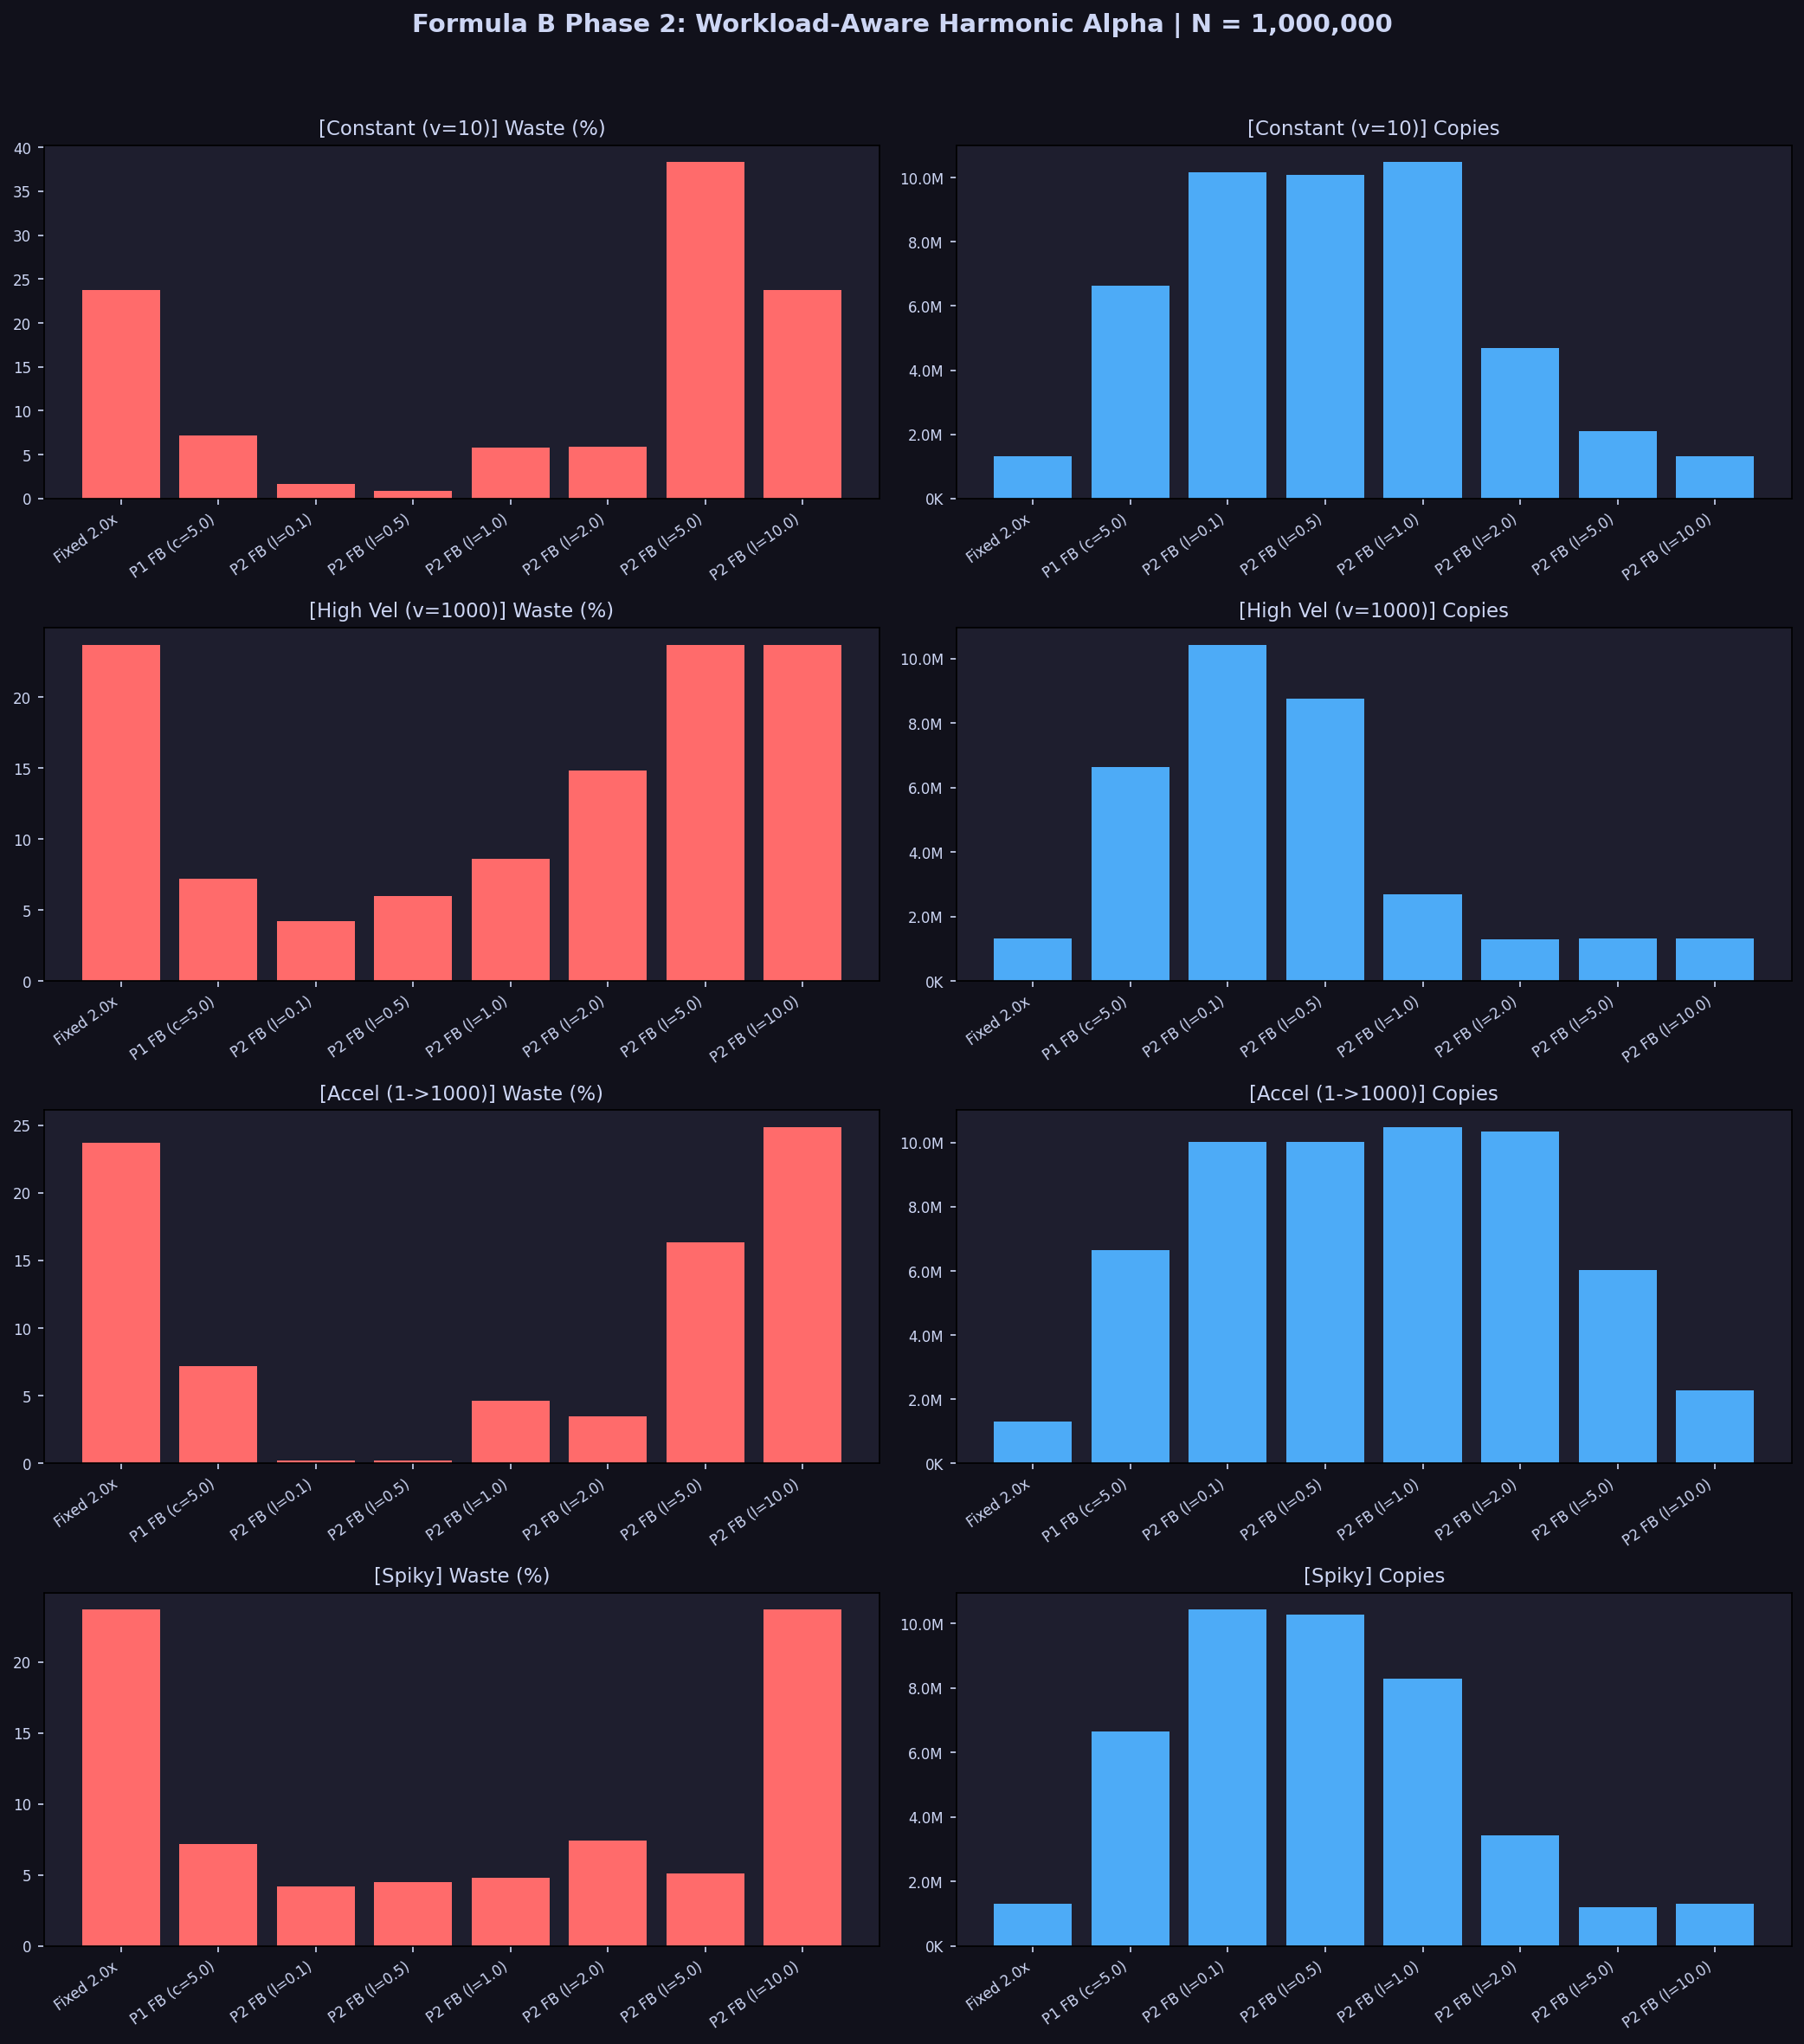
\includegraphics[width=0.9\textwidth]{../form_B_phase_2/phase2_b_comparison_1000000.png}
    \caption{Formula B Phase 2: Workload-Aware Scaling mapped across different insertion patterns at $N = 1,000,000$.}
    \label{fig:form_b_phase2_1m}
\end{figure}

The Workload-Aware Harmonic formula exhibits extraordinary performance in spiky environments. By reacting sharply to velocity jumps, $\lambda=5.0$ effectively matches the absolute minimum resize count of Fixed $2.0\times$ (17 resizes) but tightly constraints memory waste to an impressive $5.09\%$. The formula dynamically boosts its growth factor during insertion spikes and rapidly decays to conserve memory when the burst ends.

\clearpage

\section{Formula C: Weighted Capacity-History Hybrid}
Formula C blends the capacity-aware stability of Formula A with the burst-responsive history-awareness of Formula B using static weights ($w_A$ and $w_B$):
\begin{equation}
g(C,k,v) = 1 + w_A \left( \frac{3.0+2.0\ln(1+v)}{\ln(C+5)} \right) + w_B \left( \frac{1}{k} \right)
\end{equation}

\subsection{Results Summary (N = 1,000,000)}
The hybrid formula was tested across Capacity-Oriented ($0.8/0.2$), Balanced ($0.7/0.3$), and Burst-Oriented ($0.6/0.4$) configurations.

\begin{table}[h!]
    \centering
    \begin{tabular}{llrrr}
        \toprule
        \textbf{Pattern} & \textbf{Strategy} & \textbf{Resizes} & \textbf{Total Copied} & \textbf{Waste (\%)} \\
        \midrule
        \textbf{Accel ($1 \to 1000$)} & FA P2 ($k=1.0$) & 30 & 3,360,877 & 6.66\% \\
        & FB P2 ($\lambda=5.0$) & 40 & 6,040,072 & 16.37\% \\
        & FC ($0.8/0.2$) & 30 & 3,227,434 & 5.05\% \\
        \midrule
        \textbf{Spiky} & FA P2 ($k=1.0$) & 21 & 2,572,485 & 12.16\% \\
        & FB P2 ($\lambda=5.0$) & 17 & 1,209,830 & 5.09\% \\
        & FC ($0.8/0.2$) & 20 & 2,547,920 & 24.82\% \\
        \bottomrule
    \end{tabular}
    \caption{Key Performance Metrics for Formula C at 1,000,000 Insertions.}
    \label{tab:form_c}
\end{table}

\begin{figure}[h!]
    \centering
    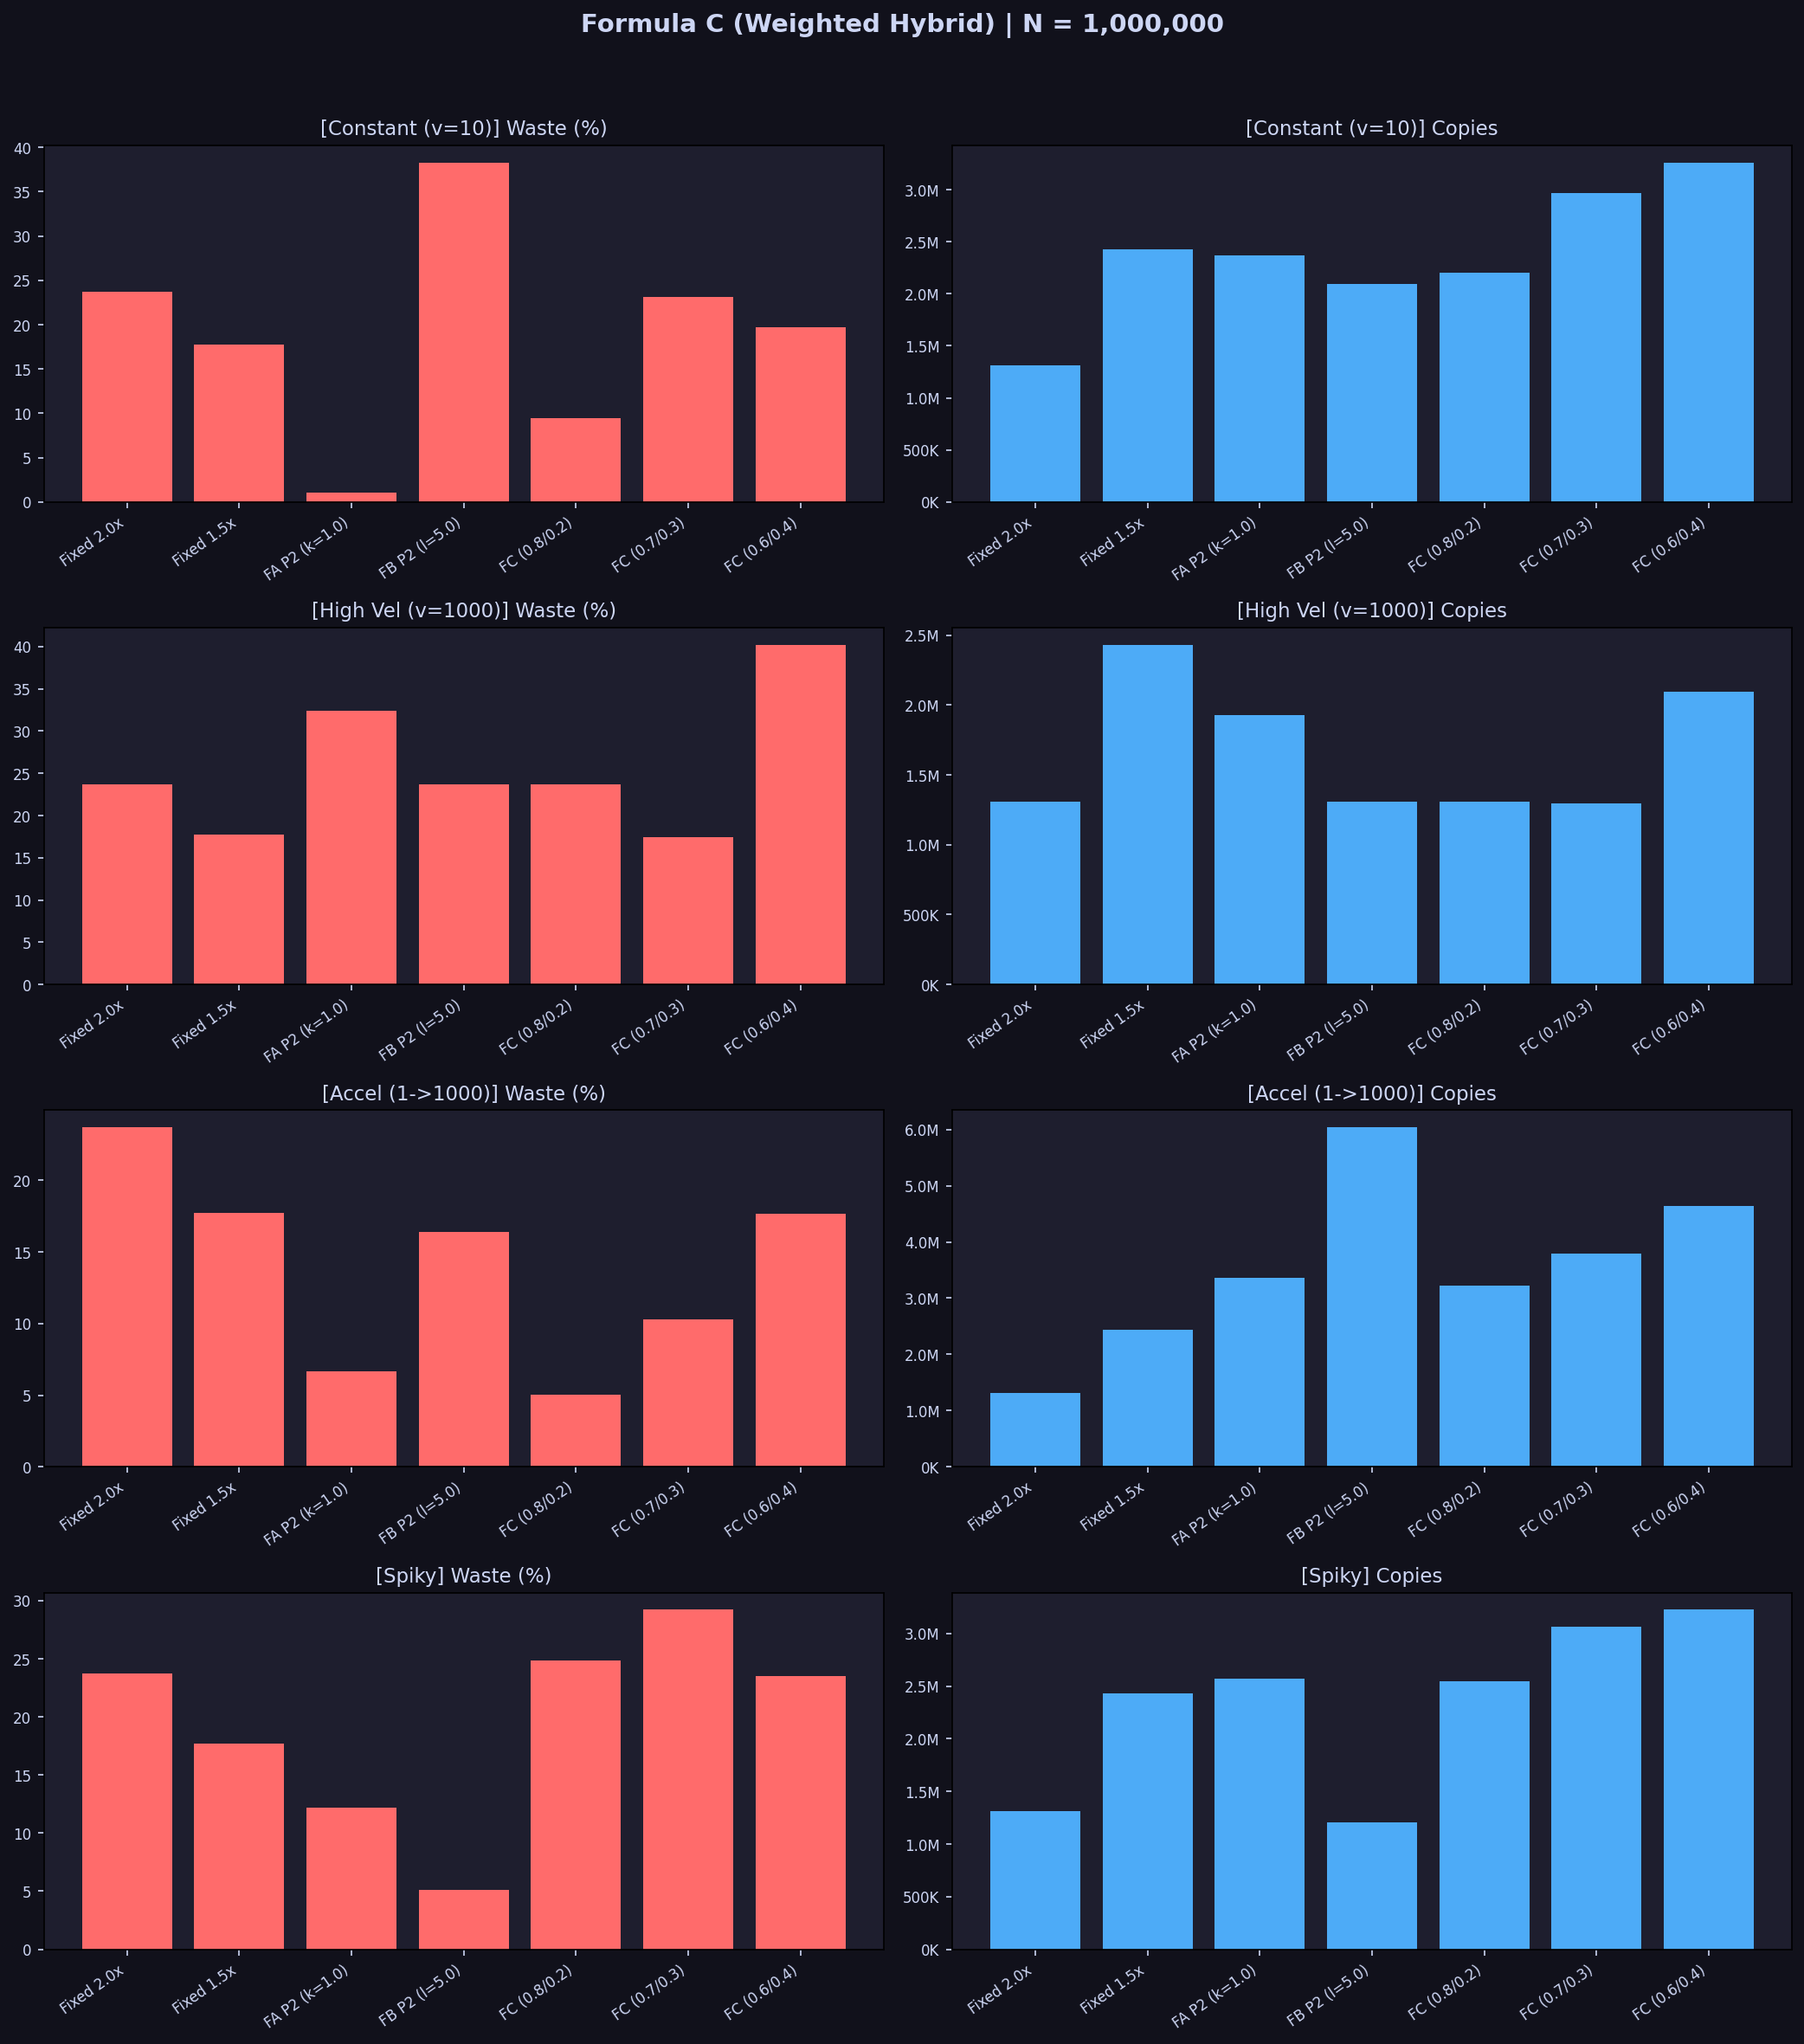
\includegraphics[width=0.9\textwidth]{../form_C_hybrid/formula_c_comparison_1000000.png}
    \caption{Formula C: Weighted Hybrid Scaling mapped across different insertion patterns at $N = 1,000,000$.}
    \label{fig:form_c_1m}
\end{figure}

The Capacity-Oriented configuration ($w_A=0.8, w_B=0.2$) successfully optimized Formula A during Accelerating workloads, achieving fewer copies and lower memory waste ($5.05\%$). However, under Spiky conditions, the static weights severely dampened the burst-responsiveness of Formula B, resulting in unacceptably high memory waste ($24.82\%$). This validates the need for \textbf{Formula D (Dynamic Weight Hybrid)}, which aims to shift weights dynamically based on workload intensity.

\clearpage

\section{Formula D: Dynamic Weight Hybrid}
Formula D addresses the rigidity of Formula C by introducing a dynamic weight function $w(v)$ that automatically shifts the growth model based on real-time insertion velocity:
\begin{equation}
w(v) = \frac{\ln(1+v)}{\ln(1+v) + s}
\end{equation}
\begin{equation}
g(C,k,v) = 1 + w(v)\left(\frac{1+\lambda\ln(1+v)}{k}\right) + (1-w(v))\left(\frac{\alpha}{\ln(C+\beta)}\right)
\end{equation}

\subsection{Results Summary (N = 1,000,000)}
By utilizing smoothing constants $s=3.0, 5.0,$ and $10.0$, Formula D actively shifts its behavior, favoring Formula A during steady state and Formula B during intense bursts.

\begin{table}[h!]
    \centering
    \begin{tabular}{llrrr}
        \toprule
        \textbf{Pattern} & \textbf{Strategy} & \textbf{Resizes} & \textbf{Total Copied} & \textbf{Waste (\%)} \\
        \midrule
        \textbf{Spiky} & FB P2 ($\lambda=5.0$) & 17 & 1,209,830 & 5.09\% \\
        & FC ($0.8/0.2$) & 20 & 2,547,920 & 24.82\% \\
        & FD ($s=5.0$) & 21 & 2,686,552 & 10.79\% \\
        \bottomrule
    \end{tabular}
    \caption{Performance Comparison for Spiky Workload at 1,000,000 Insertions.}
    \label{tab:form_d_spiky}
\end{table}

\begin{figure}[h!]
    \centering
    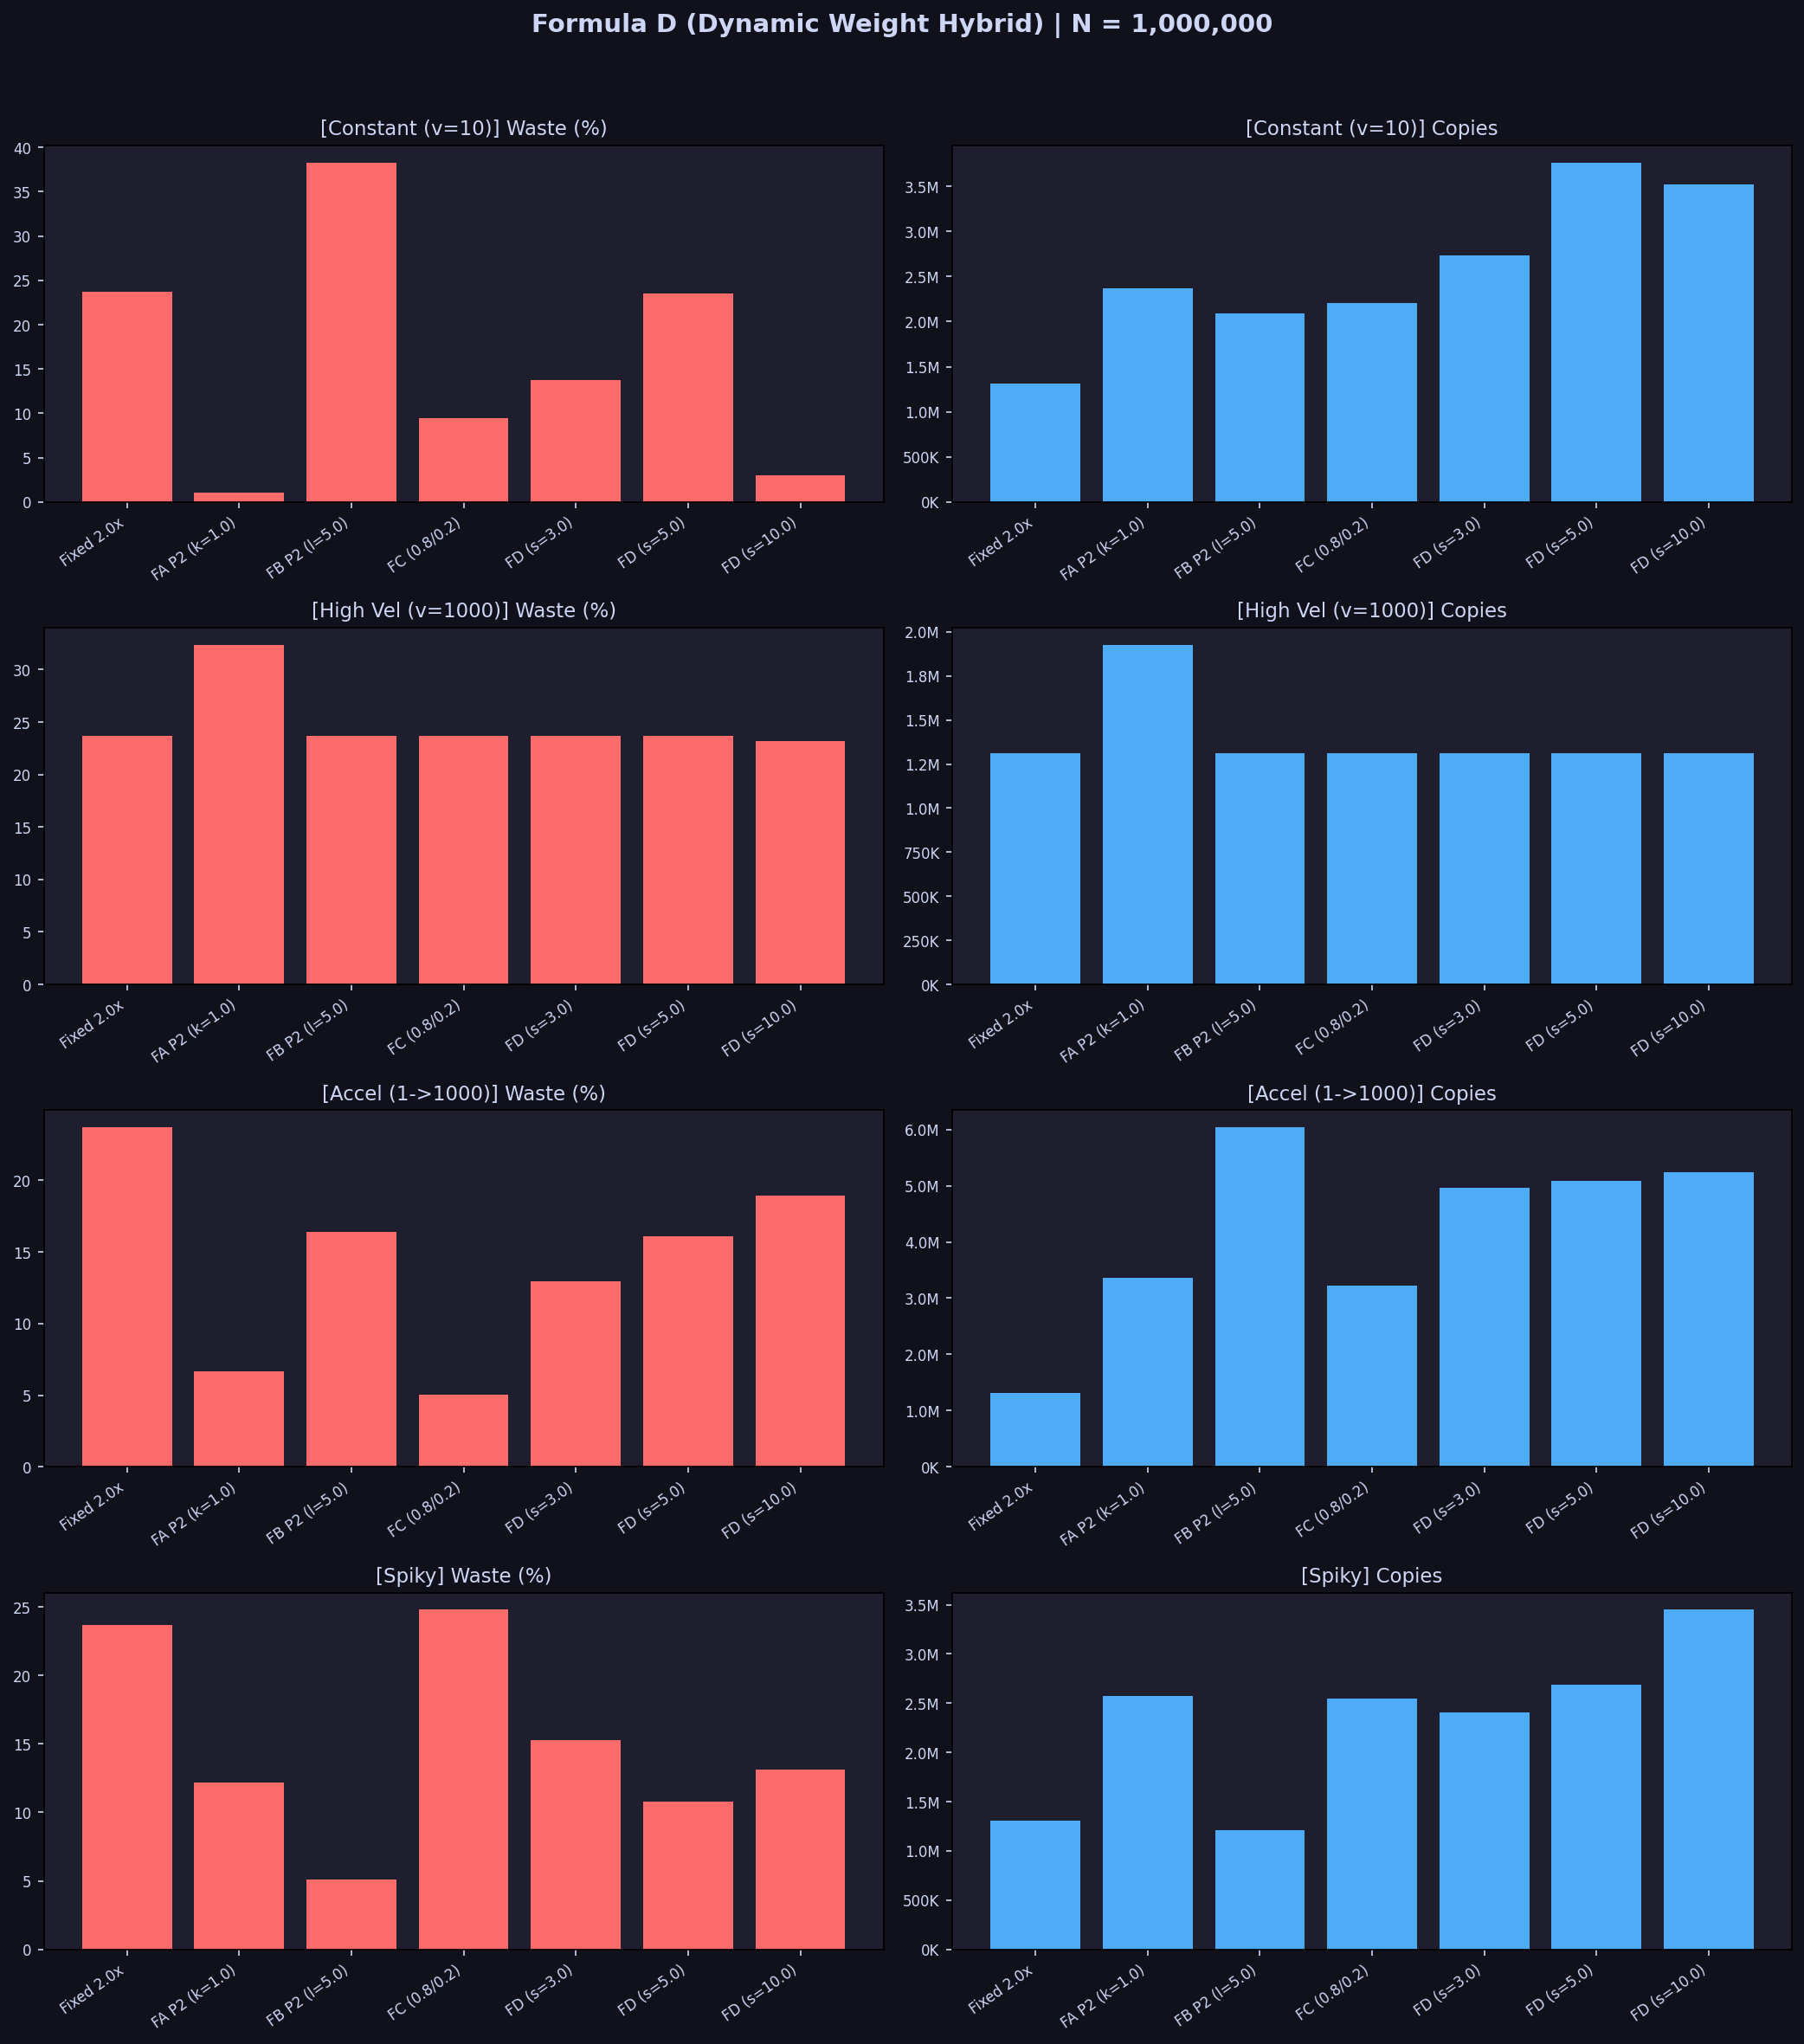
\includegraphics[width=0.9\textwidth]{../form_D_hybrid/formula_d_comparison_1000000.png}
    \caption{Formula D: Dynamic Weight Hybrid Scaling mapped across different insertion patterns at $N = 1,000,000$.}
    \label{fig:form_d_1m}
\end{figure}

The dynamic shift function successfully rescues the model from the memory bloat observed in Formula C. Under spiky conditions, Formula D dynamically shifts its weight to heavily favor the harmonic sequence, cutting the memory waste by more than half (down to $10.79\%$). While it does not reach the absolute mathematical limits of pure Formula B under pure bursts, Formula D represents an incredibly robust, fully-autonomous dynamic array growth strategy that gracefully navigates all workloads without manual parameter tuning.

\section{Conclusion}
This research demonstrates that adaptive growth factors can successfully replace fixed multipliers in dynamic arrays. Formula A provides an excellent all-around logarithmic baseline, while Formula B Phase 2 yields the ultimate solution for elastic, memory-efficient burst handling. 

\end{document}
